\subsection{Optimize the Classifier}
%The measures for evaluating the classifier are best if they are combined. 

The measures for evaluation are used to determine how well a classifier performs and to determine how the classifier could be optimized to perform better. A perfect classifier categorizes all documents to their most describing classes without classifying documents to classes they don't belong to. Figure \ref{fig:perfect_classifier} illustrates a perfect classifier which classify all documents to their correct classes. The classification results can be seen in table \ref{tab:results_perfect_classifier}.


%This is a difficult task, and we want the classifier to achieve high scores in the evaluation.
\begin{comment}
\begin{figure}[h]
\centering
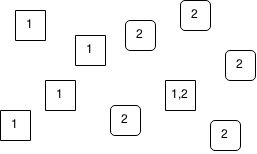
\includegraphics[width=.7\textwidth]{Chapters/Methods/All_classes}
\caption{Caption}
\label{fig:my_label}
\end{figure}

\begin{table}[h]
\centering
\renewcommand{\arraystretch}{1.25}
\begin{tabular}{c|l}
\multicolumn{2}{c}{\textbf{Number of elements in the class}} \\ \hline
\textbf{Class 1} & 5 \\ \hline
\textbf{Class 2} & 6
\end{tabular}
\\[10pt]
\caption{Caption}
\label{tab:my_label}
\end{table}

\end{comment}

\begin{figure}[h]
\centering
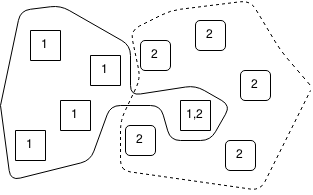
\includegraphics[width=0.7\textwidth]{Chapters/Methods/Perfect_classifier}
\caption{Illustration of a perfect classifier.}
\label{fig:perfect_classifier}
\end{figure}

\begin{table}[h]
\centering
\renewcommand{\arraystretch}{1.25}
\begin{tabular}{c|l|l|l}
\multicolumn{4}{c}{\textbf{Perfect classifier: results}} \\ \hline
\textbf{TP} & 5 &\textbf{Precision} & 1 \\ \hline
\textbf{TN} & 5 &\textbf{Recall} & 1 \\ \hline
\textbf{FP} & 0 &\textbf{Accuracy} & 1 \\ \hline
\textbf{FN} & 0 &\textbf{$F_{1}$-score} & 1
\end{tabular}
\caption{Classification results for class 1 for a perfect classifier.}
\label{tab:results_perfect_classifier}
\end{table}

\subsubsection{Why we need more than one measure for evaluation}
Creating a perfect classifier is difficult, and it is difficult to determine if the classifier perform well. The different measurements for evaluation are best when they are combined (as $F_{1}$-score), because accuracy, precision and recall can be have good results separately even if the classifier is far from perfect.  

Figure \ref{fig:high_precision}) and \ref{fig:high_recall}) illustrates classifiers that have respectively high precision and high recall. Their results can be found in table \ref{tab:results_bad_classifiers} where we can see that high precision can be found by classifier that only retrieved a few results and high recall is found for classifiers that retrieve many results. Thus, a good classifier should be neither of these, but instead balance the results. 


\begin{figure}[h]
\centering
\begin{subfigure}[b]{0.6\textwidth}
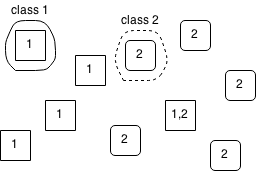
\includegraphics[width=\textwidth]{Chapters/Methods/High_precision}
\caption[Illustration of bad classifier with high precision]{Classifier A: Illustration of bad classifier with high precision.}
\label{fig:high_precision}
\end{subfigure}
\\[10pt]
\begin{subfigure}[b]{0.7\textwidth}
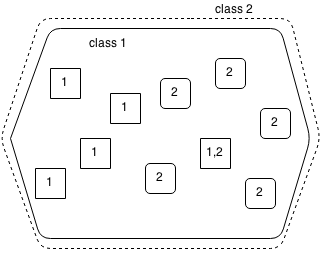
\includegraphics[width=\textwidth]{Chapters/Methods/High_recall}
\caption[Illustration of bad classifier with high recall]{Classifier B: Illustration of classifier with high recall.}
\label{fig:high_recall}
\end{subfigure}
\end{figure}


\begin{table}[h]
\centering
\renewcommand{\arraystretch}{1.25}
%\begin{tabular}{c|l|l|l|l}
%\multicolumn{2}{c}{\textbf{Classifier A}} & Classifier B \\ \hline
\begin{tabular}{l|l|l|l|l|l|l|l}
\multicolumn{4}{l}{{\bf Classifier 1}} & \multicolumn{4}{l}{{\bf Classifier2}} \\ \hline
\textbf{TP}     & 1     & \textbf{Precision}     &  1   & \textbf{TP}     & 5     & \textbf{Precision}    &   0.5  \\\hline
\textbf{TN}     & 5     & \textbf{Recall}        &  0.2   & \textbf{TN}    & 0     & \textbf{Recall}       & 1    \\\hline
\textbf{FN}     & 4     & \textbf{Accuracy}      &  0.6   & \textbf{FN}     & 5     & \textbf{Accuracy}     & 0.667    \\\hline
\textbf{FP}     & 0     & \textbf{$F_{1}$-score}      &  0.333   & \textbf{FP}     & 0     &  \textbf{$F_{1}$-score}             &    0.667
\end{tabular}
\caption{Evaluation of classifier A and B for class 1. }
\label{tab:results_bad_classifiers}
\end{table}

\begin{comment}
\begin{table}[h]
\centering
\renewcommand{\arraystretch}{1.25}
\begin{tabular}{c|l|l}
%\multicolumn{2}{c}{\textbf{Classification results for class 1}} \\ \hline
& \textbf{Classifier A} & \textbf{Classifier B} \\ \hline
\textbf{Precision} & 1 &  \\ \hline
\textbf{Recall} & 5 \\ \hline
\textbf{Accuracy} & 0 \\ \hline
\textbf{$F_{1}$-score} & 4
\end{tabular}
\caption{Caption}
\label{tab:results_high_precision}
\end{table}
\end{comment}

\begin{comment}
It is not enough to classify all documents in a class to the correct class. A perfext alskd
A classifier which categorizes all documents in a class to 
A perfect classifier categorizes all documents to the right class. We have created a classifier which might classify documents to more than one class. 
the correct results and none of the incorrect ones. 
This is a difficult task, so we try to optimize the classifier so that it retrieves most of the correct results without starting to 

The best classifier should be a classifier that retrieves m

Example of a bad classifier: It categorizes all sports article to the class sports, but also all non-sport articles to the class sport. The 

\end{comment}